\section*{\centering Kastparabel med och utan luftmotstånd}

Utan luftmotstånd...
\begin{equation} \label{eq:xyt}
    \begin{cases}
        x(t) = x_0 + v_{0,x}t \\
        y(t) = y_0 + v_{0,y}t - \dfrac{1}{2}gt^2
    \end{cases}
\end{equation}
Anta att startpunkt ($x_0$,$y_0$) ligger i (0,0) och separera $v_0$ 
\begin{align}
    x(t) &= v_0cos\theta t \label{eq:xt}\\
    y(t) &= v_0sin\theta t - \dfrac{1}{2}gt^2 \label{eq:yt}
\end{align}

\begin{figure}[H]
    \centering
    \captionsetup{justification=centering,margin=2cm}
    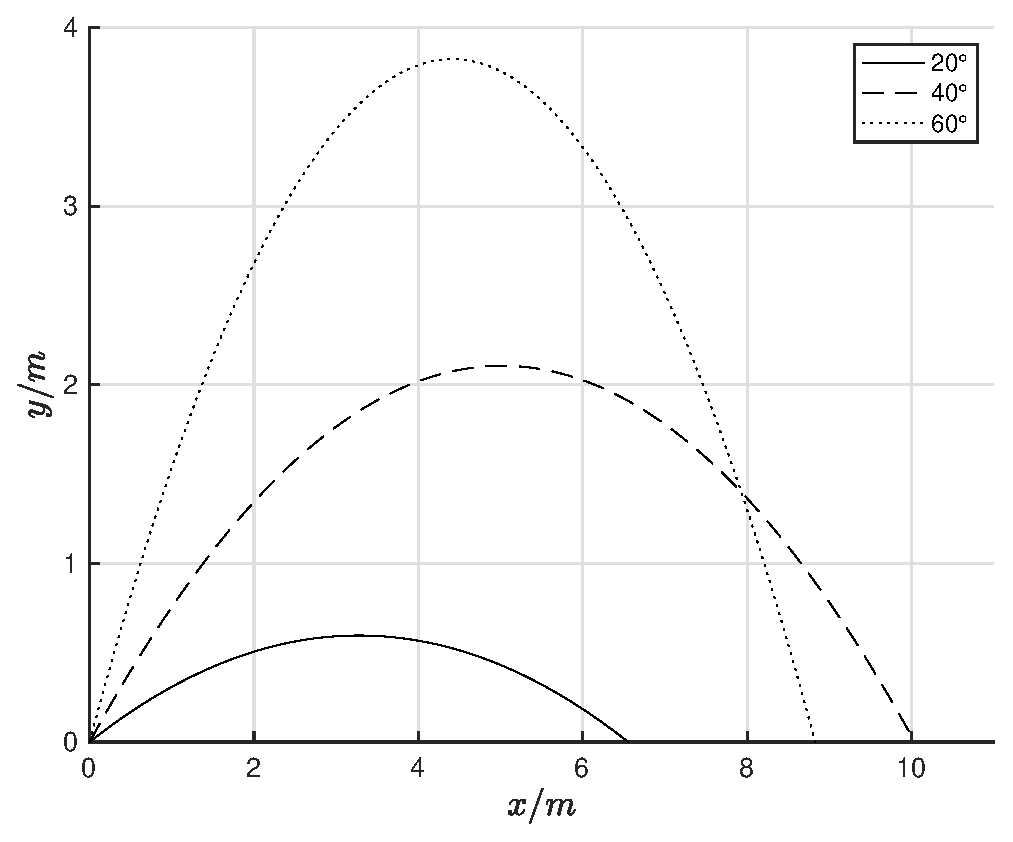
\includegraphics[scale=0.5]{Resources/Graphics/fig2_1.eps}
    \caption{BESKRIVNING}
    \label{fig:2_1}
\end{figure}

\np
\subsection*{MatLab kod}
\lstinputlisting[caption={\quad}] {Resources/Code/2.m}